\chapter{Future work}
In this section, we discuss the future directions and improvements to our current prototype that we intend to pursue in future work.

\subsection{End-to-end web application debloating}
In this work, we showed that web application debloating has the potential to significantly reduce the attack surface despite the challenges involved. Next, we discuss some of these challenges and propose directions for our future work on this topic.

\subsubsection{Handling calls to removed code}
One of the biggest challenges of using debloating in production applications is handling calls to removed functions. In our current implementation, upon executing a function that leads to debloated code, the requested operation is terminated. Then the user is notified that the intended functionality has been removed. This can happen after clicking on a link, or after several steps into filling a multi-step form. To make this more user friendly and enable website administrators to make the final decision, we envision several improvements:
\begin{itemize}

\item Adding the functionality to dynamically reintroduce the removed
code. This decision can be made either through an administration panel, or
after a second factor of authentication for privileged users. For that, we
need to identify high-risk actions and enforce further security mechanisms
and identity verification steps before continuing. From another point of
view, this step can be seen as an anomaly detection system based on history
of the user behavior.

\item Our current hypothesis is based on the observation that not all users of
an application require all features. To go one step further, one can pursue,
user-based and role-based debloating. Under this scenario, different sets of users
for the same web application are provided with their own debloated versions
based on their activity history.
\end{itemize}

\subsubsection{Propagating debloating changes to the UI}
Our current debloating setup will show error messages to users, when
they execute removed code. By disabling UI elements that exercise the
removed features we can proactively stop users from running into these
errors. Specifically, by tracking web application UI elements back to their
implementation and doing a backward traversal on the call graph, we can build
this dependency chain and disable/limit/modify UI elements. This will warn
users about the disabled features before investing any time and effort on
that function.

\begin{figure}[t]
  \centering
  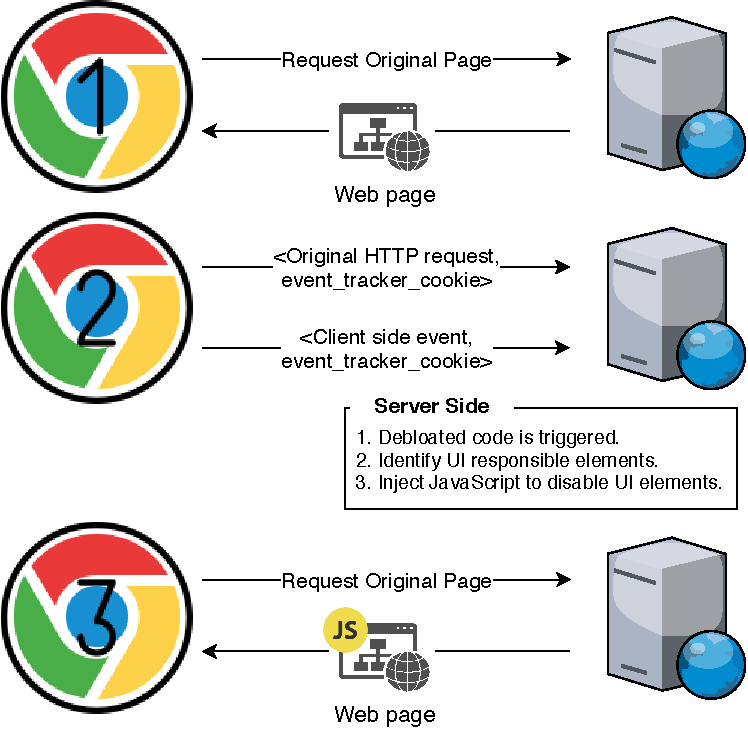
\includegraphics[width=0.7\linewidth]{figures/UI-backend-debloating.pdf}
  \caption{Overview of steps required to detect and remove UI elements for debloated actions.}
  \label{fig:uidebloating}
\end{figure}

\paragraph{Implementation details:} Web applications consist of two main components, server side and client side. Client-side code runs on users' browsers and generates HTTP requests based on user interactions with HTML and JavaScript components on the page. From server's point of view, generation of HTML content and events received from the browser are totally disconnected. The goal is to build this bridge and track server-side events as the result of client-side interactions with minimal reliance on specific application architectures.

Figure~\ref{fig:uidebloating} depicts the browser interactions required to detect and disable debloated actions on client side. Initially, PHP code is injected into all pages of the web application to add tracker cookies that are sent along page events that are reported to the server. During the first user interaction with the page at step 2 (e.g., Form submission, click on a link, etc.), by correlating the events and UI elements that triggered the request through the cookie values, we will be able to find elements and forms that trigger debloated events. The next time users request the same page, at step 3, the elements that triggered debloated actions are disabled through injected JavaScript.

\subsubsection{Code coverage collection in production environments}
By shipping the code coverage collection infrastructure to real-world users and website owners, we can gain insights into how the applications are used by different types of users.

\paragraph{Optimized code coverage collection:} To make code coverage recording less resource intensive, we need to know the source of this overhead.
Our toolset is built on top of XDebug PHP extension. To collect line level code coverage, XDebug hooks into various PHP opcodes. This makes the program execution slower and more resource intensive. Meanwhile, we only need function coverage information in our setup. This information can either be collected by a light-weight code profiler that is optimized for this task, or by developing and including PHP libraries in web applications that collect execution traces from call stack. To that end, we plan to develop optimized code profilers that can be easily installed and integrated with web applications without the need to enable PHP extensions and undergo significant performance overhead. Furthermore, by relying on function coverage instead of line coverage, our code coverage information will be more resilient to small changes that affect the order of source line numbers.

To further reduce the overhead, one can only record the code coverage for functions that include sensitive API calls (e.g., Filesystem and database interaction, dynamic code execution, network connections, etc.). The first step is to identify such functions, and through static analysis, identify code paths that interact with these APIs. By only tracking the code coverage on these specific functions, we can still reap the benefit of debloating without the associated high overheads of existing code profilers.

\subsubsection{Attack surface reduction through API specialization}
In the context of web application security, Runtime Application Self Protection (RASP) is a suite of tools and techniques that has been increasing in popularity in the recent years. By adding a defensive layer that detects attacks from within the application, the protection engine has access to execution context. This extra information increases the precision of the protection engine in detecting attacks.

A similar idea can be applied to debloating web applications. When normal users interact with a web application, functions and APIs are invoked with specific sets of parameters. By dynamically generating and enforcing whitelists that only allow benign invocation of security critical APIs, we can block exploitation attempts and reduce the attack surface and exploitability of our software.

As a motivating example, we look at the following SQL injection vulnerability in AutoSuggest 0.24 WordPress plugin~\cite{autosuggest_vulnerability}:

\begin{figure}[t]
\begin{lstlisting}[frame=single, caption={PHP code from AutoSuggest WordPress plugin with SQL injection vulnerability},captionpos=b, label={listing:autosuggest_sqli}]
<?php
$wpas_keys = $_GET['wpas_keys'];
$pageposts = $wpdb->get_results("SELECT * FROM $wpdb->posts
WHERE (post_title LIKE '%$wpas_keys%') AND post_status = 'publish' ORDER BY post_date DESC");
\end{lstlisting}
\end{figure}

Benign queries in Listing~\ref{listing:autosuggest_sqli} only target \$wpdb.posts table, whereas an exploit will likely target other tables via subqueries and UNION and try to access users table and extract information. Notice that \$wpdb.posts variable comes from WordPress configuration file and is static for each installation of WordPress.
By running each query under a different user that has the minimal permissions that satisfy the benign invocations of target query (e.g., by limiting the target table for a given query), the exploit attempt will fail.
So in this example, the query would run under the automatically generated user named ``wp\_posts\_user'' which only has ``SELECT'' permission to WordPress ``posts'' table. This would limit the exploit to be able to extract information only from posts table.

To implement this idea, we would start by creating a list of security critical PHP functions.
For each critical API, we distinguish benign and malicious invocations at runtime by learning from application usage and create a whitelist that is dynamically generated and enforces conditions to minimize the set of possible invocations of these APIs.

More concretely, we distinguish the following cases:
\begin{itemize}
  \item \textbf{Database Operations:} In the context of database operations, we limit type of operation (e.g., SELECT query) and target tables (e.g., Posts table) and database (WordPress db) for each database interaction. This can be implemented as a proxy between the database and the application or by modifying the database layer within the application (e.g., modifying the ORM). This modified API should dynamically learn and decide how the api is called and what rules should be enforced.
  \item \textbf{File System Interactions:} For these APIs, we enforce target directories, allowed file extensions and their permissions. For example, if the code writes to the file system, we dynamically learn the target directory and type/permission of files submitted through this API.
  Another possible variation is to mount virtual directories that are not directly accessible from the web, but are accessible by the PHP code itself. This prevents uploading a PHP backdoor and executing it directly from the web.
  \item \textbf{Limiting Available APIs:} By limiting the set of PHP APIs that are available to each PHP file, we can block potential exploits. For example, the login.php file should not interact with the file system or call ``eval'' or ``exec''.
\end{itemize}
